\subsection*{Модель международной торговли}
\addcontentsline{toc}{subsection}{Модель международной торговли}

\textbf{Задание:}\\
Провести численный анализ модели взаимодействия трёх экономик в среде AnyLogic.\\

\textbf{Решение:}\\
Рассмотрим упрощенную модель международной торговли между экономиками. Покажем, что международная торговля между экономиками, в которых наблюдаются предельные циклы, может привести к появлению странного аттрактора и, следовательно, возникновению хаоса.\\

Международную торговлю в некотором смысле можно рассматривать как взаимодействие изолированных экономик. Лоренцем (1987) предложена следующая модель. Рассмотрим три экономики (национальные, региональные или городские), каждая из которых описывается упрощенными детерминированными уравнениями Кейнса:\\

$Y$ -- доход\\
$r$ -- процентная ставка\\
$L$ -- функция спроса на деньги\\
$M$ -- постоянное номинальное денежное предложение\\
$p$ -- фиксированные цены товаров\\
$I$ -- функция спроса на инвестиции\\
$S$ -- функция сбережений\\
$\alpha, \beta > 0$ -- параметры установления

\begin{align*}
	\begin{cases}
		\dfrac{dY_i}{dt} = \alpha_i [I_i(Y_i, r_i) - S_i(Y_i, r_i)]\\[10pt]
		\dfrac{dr_i}{dt} = \beta \left[L_i(Y_i, r_i) - \dfrac{M_i}{p_i}\right]\\
	\end{cases}
\end{align*}

При вводе в изолированные системы фактора международной торговли, получим следующее преобразование исходной системы:

\begin{align*}
	\begin{cases}
		\dfrac{dY_i}{dt} = \alpha_i [I_i(Y_i, r_i) - S_i(Y_i, r_i) + Ex_i(Y_j, Y_k) - Im_i(Y_i)]\\[10pt]
		\dfrac{dr_i}{dt} = \beta \left[L_i(Y_i, r_i) - \dfrac{M_i}{p_i}\right]\\
	\end{cases}
\end{align*}

\newpage

Расширенная система состоит из трех связанных ограниченных осцилляторов. Как показано Ньюхаусом, Рюэлем и Такенсом (1978), возмущение движения по трехмерным торам может привести к странному аттрактору. Очевидно, что существование странного аттрактора подразумевает хаотичность траекторий. Таким образом, в модели международной возможно существование странных аттракторов.\\

Если все три автономные экономики принадлежат к осцилляторному типу, введение международной торговли может привести к существованию странного аттрактора в объединенной экономике. Существование хаотических траекторий в соответствующих моделях можно установить численным моделированием.\\

В соответствии с формулами, данная модель была реализована в среде моделирования AnyLogic. (Рисунок \ref{fig:three_economics1})
\begin{figure}[h]
	\centering 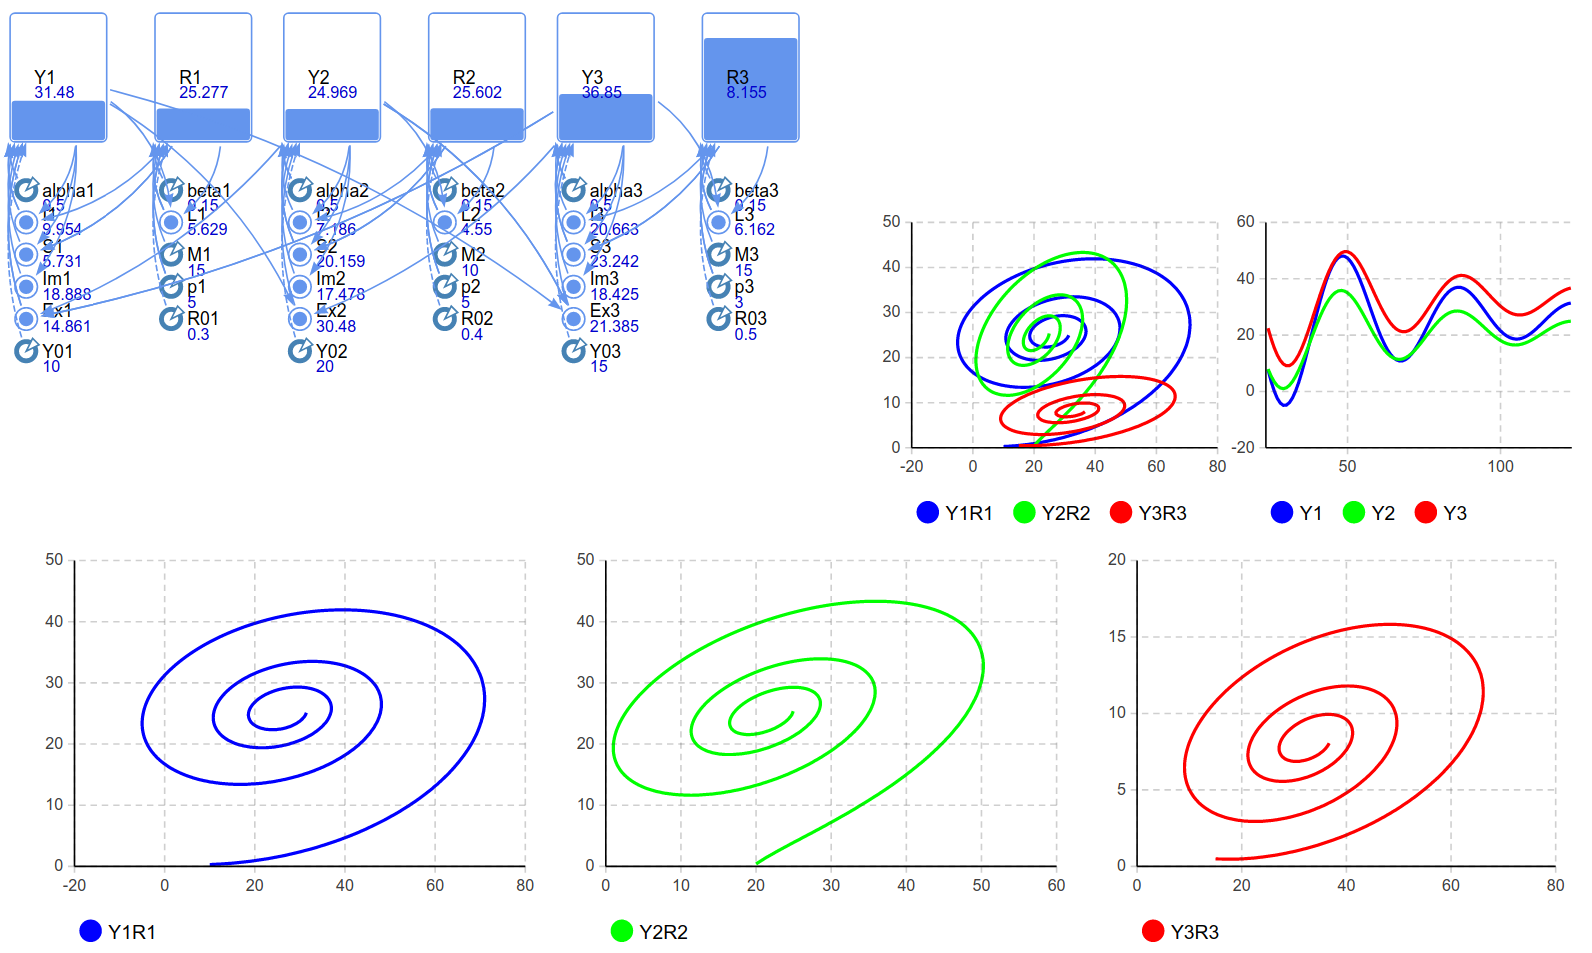
\includegraphics[scale=0.25]{three_economics1}
	\caption{Результаты построения модели международной торговли в AnyLogic}
	\label{fig:three_economics1}
\end{figure}

Таким образом, была реализована модель взаимодействия трёх экономик (модель международной торговли).